\section{Methodology}

\subsection{Problem Definition}

This paper focuses on time-series forecasting with exogenous variables. We adopt this setting for two reasons: first, it is widely encountered in real-world applications and is an important topic in academia~\cite{CrossLinear,TimeXer,DAG}; second, it forces the forecasting model to capture not only temporal dependencies but also variable dependencies, thereby providing a more challenging and representative evaluation setting.

Given a multivariate time series, each observation $\mathbf{x}_{t} \in \mathbb{R}^{F}$ at time $t$ contains both endogenous variable (forecasting target) and exogenous variables. Let the historical observation window be $\mathbf{X}_{t-L_{\text{in}}+1:t}  = (\mathbf{x}_{t-L_{\text{in}}+1},\mathbf{x}_{t-L_{\text{in}}+2},\dots,\mathbf{x}_{t}) \in \mathbb{R}^{L_{\text{in}} \times F}$. The forecasting objective is to learn a mapping:
\begin{equation}
\mathbf{\hat{X}}_{t+1:t+L_{\text{out}}}^{\text{endo}} = f_{\theta}\left(\mathbf{X}_{t-L_{\text{in}}+1:t}\right),
\end{equation}
where the goal is to predict the future $L_{\text{out}}$ steps of the endogenous variables based on a historical window of length $L_{\text{in}}$. In conventional forecasting frameworks, the architecture of $f_{\theta}$ is manually designed. In contrast, the proposed SE-TSA automatically creates the architecture topology through LLM-driven programmatic evolution.

\begin{nolinenumbers}
\begin{figure*}[htbp]
  \centering
  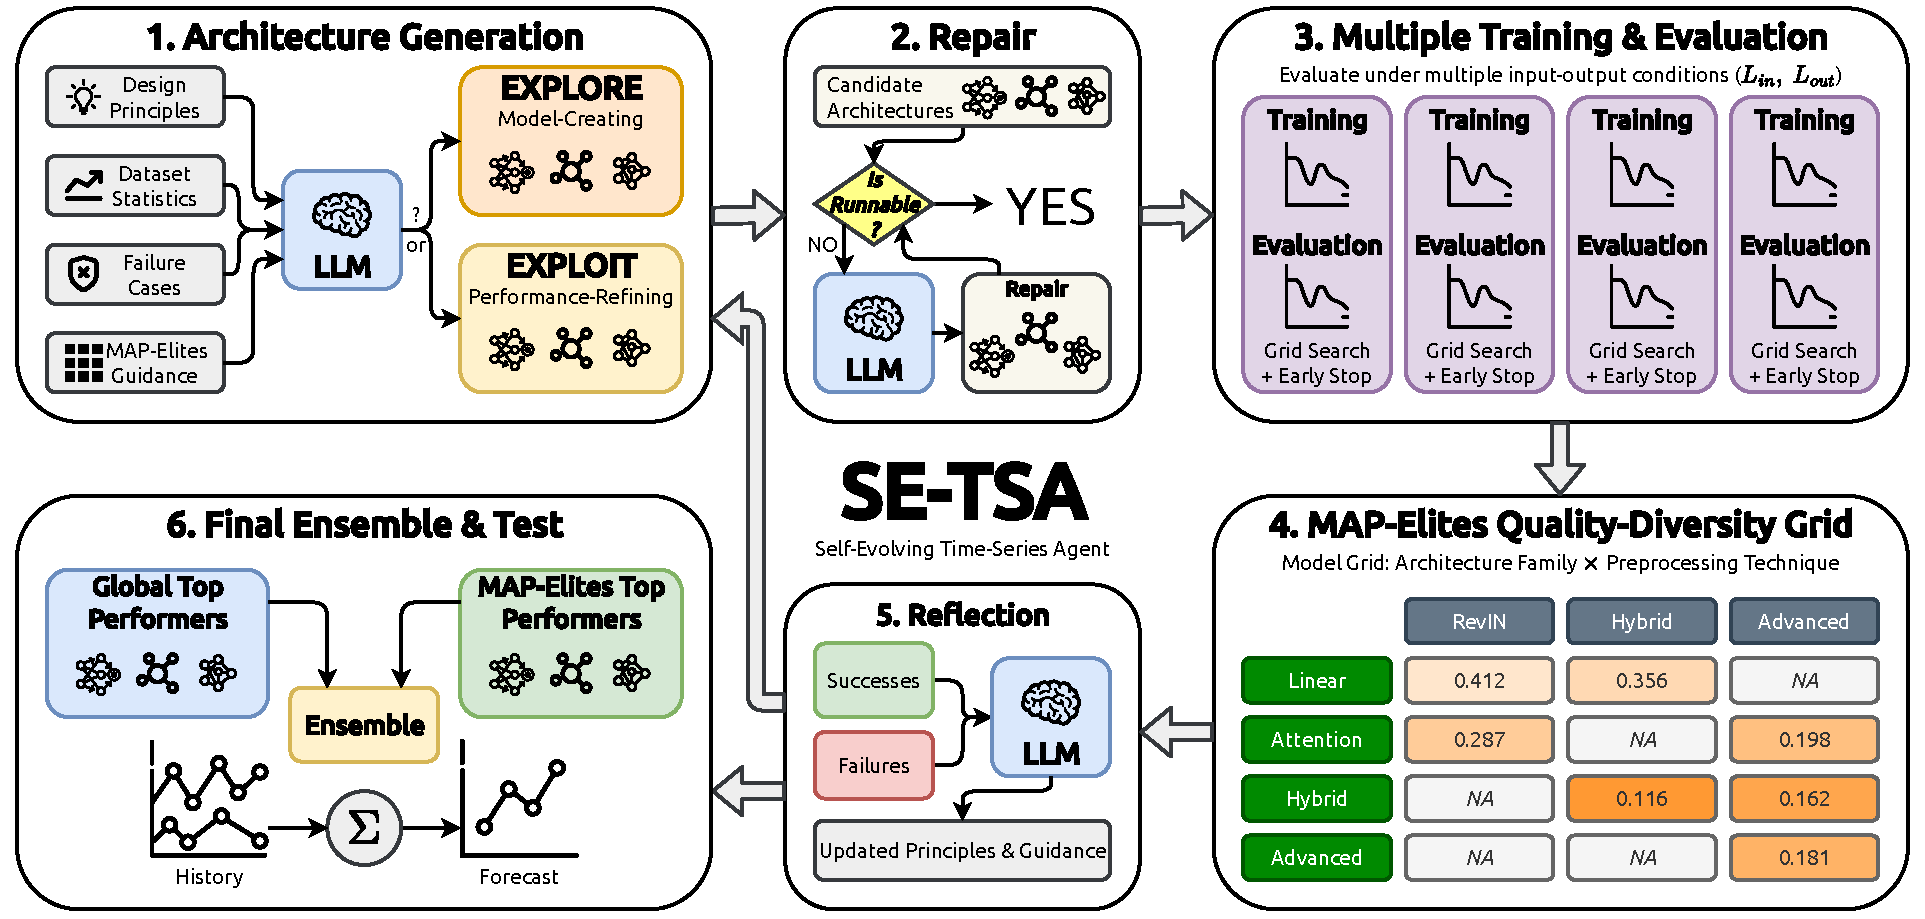
\includegraphics[width=0.98\textwidth]{figures/SE-TSA.pdf}
  \caption{Overall framework of SE-TSA. The agent system generates candidate architectures through EXPLORE/EXPLOIT dual strategies, updates the MAP-Elites quality-diversity grid after multi-condition evaluation, and accumulates interpretable design principles through a reflection mechanism, forming an iterative evolution loop.}
  \label{fig:framework}
\end{figure*}
\end{nolinenumbers}

\subsection{SE-TSA Overall Framework}

Figure~\ref{fig:framework} illustrates the overall framework of SE-TSA. Given a target dataset, SE-TSA iteratively executes the following pipeline within a predefined time budget:
\begin{enumerate}
  \item \textbf{Dual-strategy model creation}: The large language model dynamically selects either the EXPLORE strategy to create novel architectures, or the EXPLOIT strategy to refine existing high-performing architectures.

  \item \textbf{Multi-condition evaluation}: Each candidate will be validated for runnability; any non-runnable candidate will undergo a repair process. Runnable candidate models are trained and evaluated under all $(L_{\text{in}}, L_{\text{out}})$ settings. Hyperparameter search is first performed before full training.

  \item \textbf{MAP-Elites update}: Evaluated candidate models are assigned to corresponding cells in the quality-diversity grid according to their inferred architecture family and preprocessing strategy.

  \item \textbf{Reflection and principle accumulation}: After each iteration, the large language model analyzes the created models of the current round to extract design principles. Newly generated principles are deduplicated and incorporated into subsequent prompts, enabling cross-iteration meta-learning.
\end{enumerate}

After the evolutionary process terminates, representative models are selected from both the global history and the MAP-Elites archive to construct an ensemble for final forecasting.

All candidate models are trained by minimizing the mean squared error (MSE) loss between predictions and ground-truth target values:
\begin{equation}
\mathcal{L}_{\text{MSE}} = \frac{1}{T} \sum_{t=1}^{T} \left|\left| \mathbf{\hat{X}}_{t+1:t+L_{\text{out}}}^{\text{endo}} - \mathbf{X}_{t+1:t+L_{\text{out}}}^{\text{endo}} \right|\right|_{2},
\end{equation}
where $T$ denotes the number of training samples.

\subsection{Dual-Strategy Model Generation}

The model generation module is built upon an EXPLORE/EXPLOIT dual-strategy mechanism that dynamically balances architectural diversity and performance-oriented refinement. Before each iteration, the system probabilistically chooses between exploration and exploitation based on the MAP-Elites grid coverage ratio $c$ (see Section~\ref{method:map_elites}) and a decaying exploration rate $\varepsilon_t$:
\begin{equation}
p_{\text{explore}} = \max\left(\varepsilon_t, \frac{1-c}{K}\right),
\end{equation}
\begin{equation}
p_{\text{exploit}} = 1 - p_{\text{explore}},
\end{equation}
where $K$ controls the influence of grid coverage on strategy selection. The exploration rate follows an exponential decay schedule:
\begin{equation}
\varepsilon_t = \max\left(\varepsilon_{\min}, \varepsilon_{\text{base}} \cdot \gamma^t\right),
\end{equation}
where the default hyperparameters are $\varepsilon_{\text{base}}=0.9$, $\gamma=0.9$, and $\varepsilon_{\min}=0.1$. The complete generation prompts are provided in Appendix~\ref{app:prompts}.

\subsubsection{EXPLORE: Architecture Creation}

When the exploration strategy is selected, LLM is encouraged to create architectures to occupy previously unfilled regions in the MAP-Elites grid. Specifically, the system generates $N$ candidate models with diverse architectural patterns. The generation prompt incorporates four categories of information: (1) statistical summaries of the training dataset; (2) identifiers of currently unoccupied cells; (3) historically accumulated design principles; and (4) recent failure cases (e.g., unrunnable models).

By explicitly steering generation toward underexplored regions of MAP-Elite grid, the EXPLORE strategy expands the architectural diversity and improves coverage of the search space.

\subsubsection{EXPLOIT: Architecture Refinement}

When the exploitation strategy is selected, the agent system first groups models in the MAP-Elites grid according to architecture families. From each of the top-$k$ families, the model achieving the lowest loss on validation set is selected as the parent model. LLM then generates refined variants based on these information: (1) parent model specification; (2) second-best model within the same family; (3) globally best-performing model; (4) accumulated design principles; and (5) related failure cases.

Unlike EXPLORE, which emphasizes diversity expansion, the EXPLOIT strategy focuses on localized optimization while preserving the core mechanisms of validated architecture families. This enables performance refinement of occupied regions of MAP-Elite grid.

\subsection{Multi-Condition Evaluation}

Each generated candidate model first undergoes validation and automatic repair to ensure executability. Failure cases, together with their corresponding error information, are stored in a historical memory pool and used to guide future generation. Only executable candidate models proceed to the subsequent multi-condition evaluation stage.

The evaluation pipeline consists of two sequential phases:

\textbf{Configuration-space quick search}. To efficiently identify suitable hyperparameter settings, the agent system randomly samples at most $C$ candidate configurations and performs short-epoch training for each configuration. The configuration achieving the lowest validation loss is selected as the candidate configuration.

\textbf{Full training and validation}. Using the selected configuration, the candidate model is fully trained with the AdamW optimizer~\cite{AdamW} and MSE loss function.

Following the previous settings of the area~\cite{TimeMMD}, each candidate model is evaluated under multiple input--output conditions. The overall performance of a candidate model is defined as the average validation loss across all $(L_{\text{in}}, L_{\text{out}})$ conditions:
\begin{equation}
\bar{\mathcal{L}}_{\text{val}} = \frac{1}{|\mathcal{C}|}
\sum_{(L_{\text{in}}, L_{\text{out}})\in\mathcal{C}} \mathcal{L}_{\text{val}}^{(L_{\text{in}}, L_{\text{out}})},
\end{equation}
where $\mathcal{C}$ denotes the set of all input--output conditions, and $\mathcal{L}_{\text{val}}$ is MSE loss on validation set. A candidate model is allowed to replace the existing model within a MAP-Elites family only if its average validation loss $\bar{\mathcal{L}}_{\text{val}}$ is lower than that of the current one.

\subsection{MAP-Elites Quality-Diversity Grid}
\label{method:map_elites}

SE-TSA organizes evaluated candidate models within a two-dimensional MAP-Elites behavior space to jointly optimize model quality and architectural diversity. Each candidate is mapped to a behavioral region according to two discrete descriptors:

\textbf{Architecture family}: \textit{Linear}, \textit{Attention}, \textit{Hybrid}, and \textit{Advanced}, determined through code-level classification and analysis of the architectural pattern;

\textbf{Preprocessing family}: \textit{RevIN}~\cite{RevIN}, \textit{Hybrid}, and \textit{Advanced}, identified according to the employed normalization and preprocessing strategies.

The resulting behavior space contains $N_{\text{cells}} = 4 \times 3 = 12$ distinct cells. Each cell maintains the candidate model achieving the lowest validation loss within its corresponding behavioral region. Such a design, with limited expert knowledge, mitigates local optima in architectures and reduces overfitting on the validation set.

To quantify the exploration status of the search space, grid coverage is defined as the ratio between occupied cells and the total number of cells:
\begin{equation}
c = \frac{n_{\text{occupied}}}{N_{\text{cells}}},
\end{equation}
where $n_{\text{occupied}}$ denotes the number of currently populated cells.

The coverage ratio directly influences the EXPLORE/EXPLOIT decision mechanism. Specifically, low coverage increases the probability of selecting the EXPLORE strategy, encouraging the creation of architectures in underexplored behavioral regions. Conversely, high coverage shifts the search process toward EXPLOIT, allocating more computational resources to the refinement of high-performing architecture families.

\subsection{Reflection and Design Principle Accumulation}

The reflection mechanism serves as the core component enabling cross-iteration meta-learning in SE-TSA. After each iteration, the agent system identifies the best-performing and worst-performing models of the current round and constructs a reflection prompt containing complete evolutionary history, current MAP-Elites status, recent failure cases, and accumulated design principles. The complete reflection prompts are provided in Appendix~\ref{app:prompts}.

Based on this contextual information, LLM generates new design principles, which are interpretable high-level rules regarding architectural patterns, hyperparameter configurations, or preprocessing strategies.

To avoid redundant or semantically overlapping principles, each newly generated principle is encoded into a semantic embedding vector $\mathbf{p} \in \mathbb{R}^{d}$ using a BERT-like embedding model \texttt{all-MiniLM-L6-v2}~\cite{BERT,Sentence_BERT}. Cosine similarity is then computed against all previously stored principles:
\begin{equation}
\text{sim}(\mathbf{p}_{\text{new}}, \mathbf{p}_{\text{existing}}) = \frac{\mathbf{p}_{\text{new}} \cdot \mathbf{p}_{\text{existing}}}{\|\mathbf{p}_{\text{new}}\| \, \|\mathbf{p}_{\text{existing}}\|}.
\end{equation}

A newly generated principle is retained only if
\begin{equation}
\max_{\text{existing}} \text{sim}(\mathbf{p}_{\text{new}}, \mathbf{p}_{\text{existing}}) < \tau,
\end{equation}
where $\tau$ denotes the similarity threshold.

The accumulated design principles are subsequently injected into future prompts. This mechanism enables SE-TSA to progressively leverage cross-iteration induced domain knowledge during architecture creation, rather than relying solely on numerical information of data and architectures.

\subsection{Ensemble Prediction}

After the evolutionary process terminates, the final forecasting results are predicted through an ensemble module. Ensemble members are selected from two complementary candidate pools:

\textbf{Global-best pool}: the top-$N_1$ models with the lowest overall validation loss across the entire evolution process;

\textbf{Regional-best pool}: the top-$N_2$ elite models selected from different MAP-Elites behavioral regions.

Models appearing in both pools are retained with duplicated weights, thereby assigning greater influence to architectures that simultaneously achieve strong global performance and regional behavioral superiority.

Before inference, each selected ensemble member is retrained using the training set. The final prediction is then obtained through uniform averaging over all selected ensemble members:
\begin{equation}
\hat{\mathbf{X}}_{t+1:t+L_{\text{out}}}^{\text{ensemble}} =
\frac{1}{|\mathcal{M}|} \sum_{m \in \mathcal{M}} \hat{\mathbf{X}}_{t+1:t+L_{\text{out}}}^{(m)},
\end{equation}
where $\mathcal{M}$ denotes the set of all selected ensemble members.

By combining globally optimal models with behaviorally diverse elites, the ensemble strategy improves robustness and generalization ability while reducing the risk of overfitting to a single architecture family.
